\section{鞅、停止与补偿}
\label{sec:ctsp-martingales}

上一节研究给定当前状态后整个条件未来的分布；本节只看条件均值。第~\ref{chap:discrete-time-stochastic-processes}章的核心问题是：给定历史后，增量还有没有可以预知的平均漂移？没有漂移的累计量是鞅，它在停时处保持期望，最大偏差受终点矩控制，有界时还会收敛。这些结论在连续时间中都成立，但需要补上三类条件：路径要取右连续版本，停时要用离散停时逼近，积分前还常常需要局部化。计数过程还要扣掉“平均会来多少事件”这一可预测部分，才能得到鞅，这就是补偿。

\subsection{连续时间鞅与局部鞅}
\label{sec:ctsp-continuous-martingales}

\paragraph{任意两时刻的条件均值}
离散鞅的定义只比较相邻时刻：$\mathbb E[M_{n+1}\mid\mathcal F_n]=M_n$，再由塔式性质推出任意$m\leq n$的关系。连续时间没有相邻时刻，定义直接要求任意两个时刻。

\begin{definition}[连续时间鞅]
  \label{def:ctsp-martingale}
  适应过程$(M_t)_{t\geq0}$称为相对于$(\mathcal F_t)$的\term{鞅}，若每个$M_t$可积，并且对任意$0\leq s\leq t$，$\mathbb E[M_t\mid\mathcal F_s]=M_s$几乎必然。把等号换成“$\geq$”或“$\leq$”分别得到次鞅与超鞅。
\end{definition}

在满足通常条件的滤过下，每个鞅都有右连续有左极限的修改\scite{math-kallenberg2021probability}，本章总取这样的版本。由引理~\ref{lem:ctsp-right-continuous-modification}，这个版本在不可区分意义下唯一，所以“鞅的路径”是有确切意义的对象。

Brownian运动提供了几个基本的鞅。设$s\leq t$，记$\Delta=W_t-W_s$，它独立于$\mathcal F_s$且服从$\mathcal N(0,t-s)$。
\begin{itemize}
  \item $W_t$：$\mathbb E[W_t\mid\mathcal F_s]=W_s+\mathbb E\Delta=W_s$。
  \item $W_t^2-t$：$\mathbb E[W_t^2\mid\mathcal F_s]=W_s^2+2W_s\mathbb E\Delta+\mathbb E\Delta^2=W_s^2+(t-s)$。
  \item $\exp(\theta W_t-\theta^2t/2)$，$\theta\in\mathbb R$：由$\mathbb Ee^{\theta\Delta}=e^{\theta^2(t-s)/2}$，条件期望恰好抵消多出的指数因子。
\end{itemize}
第二个例子说明，$W_t^2$是次鞅，它的平均增长率正好是$1$；减去$t$以后才没有漂移。这一“减去可预测增长”的操作在计数过程上表现得更加直观。

设$N$是速率$\lambda$的Poisson过程，$\widetilde N_t=N_t-\lambda t$。增量$N_t-N_s$独立于$\mathcal F_s$，均值与方差都是$\lambda(t-s)$，同样的计算给出：$\widetilde N_t$与$\widetilde N_t^2-\lambda t$都是鞅。图~\ref{fig:ctsp-compensated-poisson}比较了扣除平均前后的路径。原始计数整体向上倾斜，补偿后的路径在每个到达时刻仍向上跳一格，在两次到达之间以斜率$-\lambda$下降；路径束围绕零散开，宽度大约按$\sqrt{\lambda t}$增长。

\begin{figure}[htbp]
  \centering
  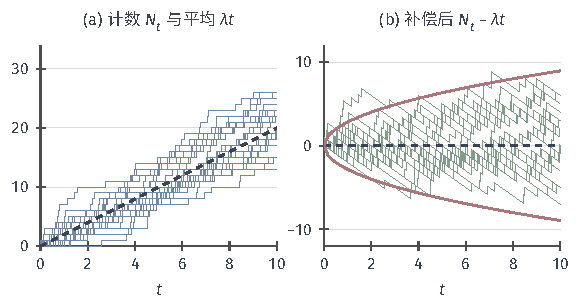
\includegraphics[width=98mm]{figures/03-optimization-evolution-and-signals/02-processes-and-trajectory-evolution/tikz/ctsp-compensated-poisson/figure.pdf}
  \caption{扣除平均累计前后的计数路径。$25$条独立的Poisson路径，速率$\lambda=2$，固定随机种子。(a)原始计数$N_t$围绕平均$\lambda t$（虚线）上升；(b)补偿后的$N_t-\lambda t$在到达时刻仍跳高一格，到达之间按斜率$-2$下降，虚线为零均值，红线为$\pm2\sqrt{\lambda t}$，即两倍标准差的解析曲线，不是置信带。}
  \label{fig:ctsp-compensated-poisson}
\end{figure}

\paragraph{局部化与局部鞅}
后面构造的随机积分$\int_0^tH_s\,\mathrm dW_s$在只知道$\int_0^tH_s^2\,\mathrm ds<\infty$几乎必然时，未必可积，于是不能直接称为鞅。处理办法与离散章的停止过程相同：用一列停时把过程截在“还受控制”的范围内，在每个截断上它是真鞅。

\begin{definition}[局部鞅]
  \label{def:ctsp-local-martingale}
  右连续适应过程$M$称为\term{局部鞅}（local martingale），若存在停时列$\rho_n\uparrow\infty$几乎必然，使每个停止过程$M^{\rho_n}_t=M_{t\wedge\rho_n}$都是鞅。这样的$(\rho_n)$称为\term{局部化}（localization）序列。
\end{definition}

“局部”指的是在随机时间范围内局部，而不是在状态空间中局部。每条路径最终会被某个$\rho_n$覆盖到任意给定的有限时刻，但这并不保证去掉截断后仍可以交换极限与期望。局部鞅不一定是鞅：在三维中，$1/\|\bm W_t+\bm x_0\|$（$\bm x_0\neq\bm0$）是局部鞅，期望却随时间严格下降\scite{math-kallenberg2021probability}。取期望之前，必须另外验证可积性。

有两类情形可以从局部鞅回到鞅或超鞅，后面都会用到。第一，若$\mathbb E\sup_{s\leq t}|M_s|<\infty$对每个$t$成立，控制收敛定理允许在$\mathbb E[M_{t\wedge\rho_n}\mid\mathcal F_s]=M_{s\wedge\rho_n}$中令$n\to\infty$，所以$M$是鞅。第二，非负局部鞅是超鞅：对$s\leq t$，由条件Fatou引理，
\[
  \begin{aligned}
    \mathbb E[M_t\mid\mathcal F_s]&=\mathbb E\bigl[\liminf_nM_{t\wedge\rho_n}\bigm|\mathcal F_s\bigr]\\
    &\leq\liminf_n\mathbb E[M_{t\wedge\rho_n}\mid\mathcal F_s]=\liminf_nM_{s\wedge\rho_n}=M_s .
  \end{aligned}
\]
非负性使Fatou引理可用；可积性也由此得到：$\mathbb EM_t\leq\mathbb EM_0$。这一事实将在第~\ref{sec:ctsp-girsanov}节判断路径权重是否保持总质量，并在第~\ref{sec:ctsp-sa-lyapunov}节构造连续时间的几乎超鞅。

\subsection{可选抽样、最大偏差与极限}
\label{sec:ctsp-optional-sampling}

\paragraph{从离散停时到连续停时}
离散章证明了有界停时的可选抽样：若$\sigma\leq\tau\leq K$，则$\mathbb E[M_\tau\mid\mathcal F_\sigma]=M_\sigma$。连续时间的证明分两步：先对式~\eqref{eq:ctsp-dyadic-stopping}的二进逼近使用离散结论，再借路径右连续和一致可积性取极限。

\begin{theorem}[连续时间的可选抽样]
  \label{thm:ctsp-optional-sampling}
  设$M$是右连续鞅，$\sigma\leq\tau$是停时，且$\tau\leq K$对某个常数$K$成立。则$M_\tau$可积，并且$\mathbb E[M_\tau\mid\mathcal F_\sigma]=M_\sigma$。特别地，$\mathbb EM_\tau=\mathbb EM_0$。
\end{theorem}

\begin{proof}
取$\sigma_n,\tau_n$为$\sigma,\tau$的二进上逼近。它们只取网格$2^{-n}\mathbb N$上的值，并且$\sigma_n\leq\tau_n\leq K+1$。在这一网格上，$(M_{k2^{-n}})_k$是离散鞅，离散可选抽样给出：对$A\in\mathcal F_\sigma\subseteq\mathcal F_{\sigma_n}$，
\[
  \mathbb E[M_{\tau_n}\mathbb I_A]=\mathbb E[M_{\sigma_n}\mathbb I_A].
\]
令$n\to\infty$。右连续性给出$M_{\tau_n}\to M_\tau$与$M_{\sigma_n}\to M_\sigma$逐点成立。离散可选抽样又给出$M_{\tau_n}=\mathbb E[M_{K+1}\mid\mathcal F_{\tau_n}]$，同一可积变量的条件期望族一致可积，所以收敛也在$L^1$中成立，可以在等式两端取极限。于是$\mathbb E[M_\tau\mathbb I_A]=\mathbb E[M_\sigma\mathbb I_A]$对所有$A\in\mathcal F_\sigma$成立，而$M_\sigma$是$\mathcal F_\sigma$可测的（渐进可测过程在停时处的取值可测），结论成立。
\end{proof}

对无界停时，定理给出$\mathbb EM_{\tau\wedge t}=\mathbb EM_0$对每个$t$成立。把$t$送到无穷要交换极限与期望，需要停止过程$(M_{\tau\wedge t})_{t\geq0}$一致可积，或被某个可积变量控制。第~\ref{sec:ctsp-strong-markov}节的首次到达时刻$\tau_a$给出了反例：$\tau_a<\infty$几乎必然且$W_{\tau_a}=a$，但$\mathbb EW_{\tau_a}=a\neq0=\mathbb EW_0$。条件不成立的地方在于停止过程$W_{t\wedge\tau_a}$向下没有界，并且$\mathbb E\tau_a=\infty$。

\paragraph{首次退出的计算}
当停止过程有界时，可选抽样可以直接用来计算。设$a<x<b$，Brownian运动从$x$出发，即考虑$X_t=x+W_t$，令$\tau=\inf\{t:X_t\notin(a,b)\}$为首次退出区间的时刻。下面逐步核对所需条件。

第一，$\tau$是停时：它是连续适应过程首次到达闭集$(-\infty,a]\cup[b,\infty)$的时刻。第二，$\tau$有限且可积。对鞅$X_t^2-t$在有界停时$\tau\wedge t$处使用定理~\ref{thm:ctsp-optional-sampling}，
\[
  \mathbb E(\tau\wedge t)=\mathbb EX_{\tau\wedge t}^2-x^2\leq\max(a^2,b^2),
\]
因为停止前$X$留在$[a,b]$中。令$t\to\infty$，单调收敛定理给出$\mathbb E\tau\leq\max(a^2,b^2)<\infty$。第三，由路径连续，$X_\tau\in\{a,b\}$。

现在对两个鞅取极限。$X_{\tau\wedge t}$取值于$[a,b]$，有界，控制收敛给出$\mathbb EX_\tau=x$。记$p=\mathbb P(X_\tau=b)$，则$pb+(1-p)a=x$，即
\begin{equation}
  \mathbb P_x(X_\tau=b)=\frac{x-a}{b-a}.
  \label{eq:ctsp-exit-probability}
\end{equation}
再对$X_t^2-t$令$t\to\infty$：$X^2_{\tau\wedge t}$有界，$\tau\wedge t$单调上升，两项分别用控制收敛与单调收敛，得到$\mathbb E\tau=\mathbb EX_\tau^2-x^2=pb^2+(1-p)a^2-x^2$。代入$p$并化简，
\begin{equation}
  \mathbb E_x\tau=(x-a)(b-x).
  \label{eq:ctsp-exit-time}
\end{equation}
例如区间$(0,1)$、起点$0.3$时，路径先到达$1$的概率为$0.3$，平均退出时间为$0.21$。第~\ref{sec:ctsp-first-passage}节会把同样的结果解释为边值问题的解。

\paragraph{最大偏差}
很多时候我们关心的不是终点误差，而是整个运行区间上最坏的偏离。离散章的Doob最大不等式控制了$\max_{k\leq n}|M_k|$；连续时间的上确界涉及不可数多个时刻，需要右连续性把它化为可数集上的上确界。

\begin{theorem}[Doob最大不等式]
  \label{thm:ctsp-doob-maximal}
  设$X$是右连续的非负次鞅，$t>0$，$\lambda>0$。则
  \[
    \lambda\,\mathbb P\Bigl(\sup_{s\leq t}X_s>\lambda\Bigr)\leq\mathbb EX_t .
  \]
  若$M$是右连续鞅且$\mathbb EM_t^2<\infty$，则$\mathbb E\sup_{s\leq t}M_s^2\leq4\,\mathbb EM_t^2$。
\end{theorem}

\begin{proof}
令$D_n=\{kt2^{-n}:0\leq k\leq2^n\}$。在有限集$D_n$上，离散Doob不等式给出$\lambda\mathbb P(\max_{s\in D_n}X_s>\lambda)\leq\mathbb EX_t$。$D_n$递增，事件$\{\max_{D_n}X_s>\lambda\}$随$n$上升到$\{\sup_{s\in D}X_s>\lambda\}$，其中$D=\bigcup_nD_n$；由右连续性，$D$上的上确界等于$[0,t]$上的上确界，因为任一时刻的取值都是$D$中从右侧逼近的点的极限。概率的单调连续性完成第一式。第二式同样先在$D_n$上使用离散的$L^2$版本（作用于非负次鞅$|M|$），再由单调收敛取极限。
\end{proof}

例如对Brownian运动，$W_t^2$是非负次鞅，第一式给出$\mathbb P(\sup_{s\leq1}|W_s|\geq3)\leq\mathbb EW_1^2/9=1/9$。由反射原理可以算出精确值至多为$4[1-\Phi(3)]\approx0.0054$，所以这个界很粗糙；它的价值在于只用终点的二阶矩就控制了整个时段，并且对任何平方可积鞅都适用。第~\ref{sec:ctsp-sde-existence}节用第二式控制Picard迭代在整个时段上的误差。

\paragraph{鞅的收敛}
最后看时间趋于无穷时的极限。离散章用上穿次数证明了：$L^1$有界的次鞅几乎必然收敛。连续时间先在可数稠密集上计数上穿，再由右连续性把结论推广到全部时刻。

\begin{theorem}[连续时间鞅收敛]
  \label{thm:ctsp-martingale-convergence}
  设$X$是右连续次鞅，且$\sup_t\mathbb EX_t^+<\infty$。则$X_t$几乎必然收敛到一个可积的极限$X_\infty$。若$M$是一致可积的右连续鞅，则还有$M_t\to M_\infty$于$L^1$，且$M_t=\mathbb E[M_\infty\mid\mathcal F_t]$；若$\sup_t\mathbb EM_t^2<\infty$，则收敛也在$L^2$中成立。
\end{theorem}

三个结论的条件各不相同，不能混用。指数鞅$Z_t=\exp(W_t-t/2)$说明了这一点：它是非负鞅，$\mathbb EZ_t=1$，满足第一个条件，所以几乎必然收敛。由于$W_t/t\to0$几乎必然（对整数时刻用强大数律，再用最大不等式控制相邻整数之间的波动），指数$W_t-t/2\to-\infty$，极限$Z_\infty=0$。期望从$1$跳到$0$，所以$Z$不一致可积，$L^1$收敛不成立。路径有极限，不等于期望也有相同的极限。

\subsection{计数补偿与累计波动}
\label{sec:ctsp-compensation}

\paragraph{常强度计数的补偿}
上一小节已经核验$\widetilde N_t=N_t-\lambda t$是鞅。把这一计算写成一般原则：计数过程$N$本身是次鞅，它的增长可以拆成两部分，一部分是事先就能预期的平均增长$\lambda t$，另一部分是事件实际何时发生带来的随机起伏。前者称为补偿量，后者是鞅。

\begin{theorem}[Poisson补偿]
  \label{thm:ctsp-poisson-compensation}
  设$N$是相对于$(\mathcal F_t)$的速率$\lambda$的Poisson过程。则$\widetilde N_t=N_t-\lambda t$与$\widetilde N_t^2-\lambda t$都是平方可积鞅。
\end{theorem}

\begin{proof}
对$s<t$，$N_t-N_s$独立于$\mathcal F_s$，均值与方差都是$\lambda(t-s)$。第一式由$\mathbb E[\widetilde N_t-\widetilde N_s\mid\mathcal F_s]=0$得到。展开$\widetilde N_t^2=(\widetilde N_s+(\widetilde N_t-\widetilde N_s))^2$，交叉项的条件期望为零，平方项的条件期望为$\lambda(t-s)$，得到第二式。
\end{proof}

\paragraph{可预测强度与补偿量}
事件速率常常随时间或状态改变。门店的顾客在午间更多；连续时间Markov链从状态$i$跳往$j$的速率为$q_{i,j}$，只在链处于$i$时才起作用。设$N$是不爆炸的计数过程，$\lambda_t\geq0$是可预测过程，并且对每个$t$，$\int_0^t\lambda_s\,\mathrm ds<\infty$几乎必然。若
\begin{equation}
  N_t-\int_0^t\lambda_s\,\mathrm ds\quad\text{是局部鞅},
  \label{eq:ctsp-intensity}
\end{equation}
就称$\lambda_t$为$N$的强度，$\Lambda_t=\int_0^t\lambda_s\,\mathrm ds$为\term{补偿量}（compensator）。确定性强度$\lambda(t)$给出非齐次Poisson过程；对连续时间Markov链，从$i$到$j$的跳跃次数$N^{i,j}_t$的强度为$q_{i,j}\mathbb I\{X_{t-}=i\}$。

式~\eqref{eq:ctsp-intensity}中的三个条件各有用途。可预测性要求强度只用严格早于当前时刻的信息，第~\ref{sec:ctsp-time-jump-integrals}节将用一个具体计算说明，若允许强度看到当次事件，零均值性质就会被破坏。不爆炸保证$N_t$有限。累计强度有限则使局部化可行：取$\rho_n=\inf\{t:N_t\geq n\text{ 或 }\Lambda_t\geq n\}$，停止后的计数与补偿量都不超过$n+1$，从而可积，鞅等式可以在每个截断上核对。

\paragraph{三种累计量}
计数过程还带来三个容易混淆的累计量。以常强度Poisson过程为例：原始计数$N_t$记录实际发生了多少事件；补偿后的$\widetilde N_t$是扣除平均增长后的噪声；描述噪声大小的又有两种量。沿路径累计跳跃的平方，得到$[\widetilde N]_t=\sum_{s\leq t}(\Delta\widetilde N_s)^2=N_t$，它是随机的；使$\widetilde N_t^2-\langle\widetilde N\rangle_t$成为鞅的可预测累计量是$\langle\widetilde N\rangle_t=\lambda t$，它是确定的。前者是实现出来的波动，后者是预先可知的波动预算，二者的期望相同。

复合Poisson过程有同样的结构。若$\mathbb E|J_1|<\infty$，$C_t-\lambda t\,\mathbb EJ_1$相对于记录到达时刻与标记的历史是鞅；若再有$\mathbb EJ_1^2<\infty$，平方跳跃累计为$\sum_{k\leq N_t}J_k^2$，可预测二阶累计为$\lambda t\,\mathbb EJ_1^2$，与式~\eqref{eq:ctsp-compound-moments}一致。例如每次理赔恒为$2$时，平均累计速率为$2\lambda$，二阶累计速率却是$4\lambda$。下一节的跳跃积分要把可预测的系数乘到这些补偿增量上，并用可预测二阶累计控制其方差。

更一般地，Doob--Meyer分解断言：满足适当一致可积条件（D类）的右连续次鞅可以唯一地写成鞅与可预测非减过程之和\scite{math-kallenberg2021probability}。计数过程的补偿是它最直观的实例。这一定理不说明任意适应过程都有这样的分解，也不保证分解出的鞅平方可积；本章只在已经核对条件的具体过程上使用补偿。
